\subsection{Results}

Global dose--response analyses indicated that LSD (Q$_M$ = 11.36, $p = 7.49\times10^{-4}$), MDMA (Q$_M$ = 15.22, $p = 1.07\times10^{-6}$), and psilocybin (Q$_M$ = 19.13, $p = 3.94\times10^{-11}$) exhibited significant session-level slopes (Table~\ref{tab:dr-global-session}). Ayahuasca could not be evaluated because only a single dosing condition was available. Across molecules, the fitted curves suggested monotonic dose increases with mild deviations from linearity (Figure~\ref{fig:dr-global-session}).

Only a subset of adverse events displayed session dose sensitivity for each molecule (Figure~\ref{fig:dr-by-ae-session}). Headache, nausea, and illusions increased with LSD exposure; MDMA amplified nausea, headache, dizziness, and fatigue; and psilocybin was associated with higher rates of fatigue and hypertension (Table~\ref{tab:dr-ae-by-molecule-session}).

Session-to-follow-up forest comparisons confirmed that psilocybin and ayahuasca were only estimable during dosing sessions, whereas LSD and MDMA had additional follow-up panels (Figure~\ref{fig:forest-combined}). All significant AE signals were transient: LSD showed session-limited elevations in nausea, headache, and illusions; MDMA effects on nausea, dizziness, headache, and fatigue faded after dosing; and psilocybin produced session-only hypertension and fatigue (Table~\ref{tab:forest-ae-by-window}). The tally of transient versus persistent or emergent signals is summarized in Table~\ref{tab:forest-ae-sig-counts}.

\begin{figure}[htb]
  \centering
  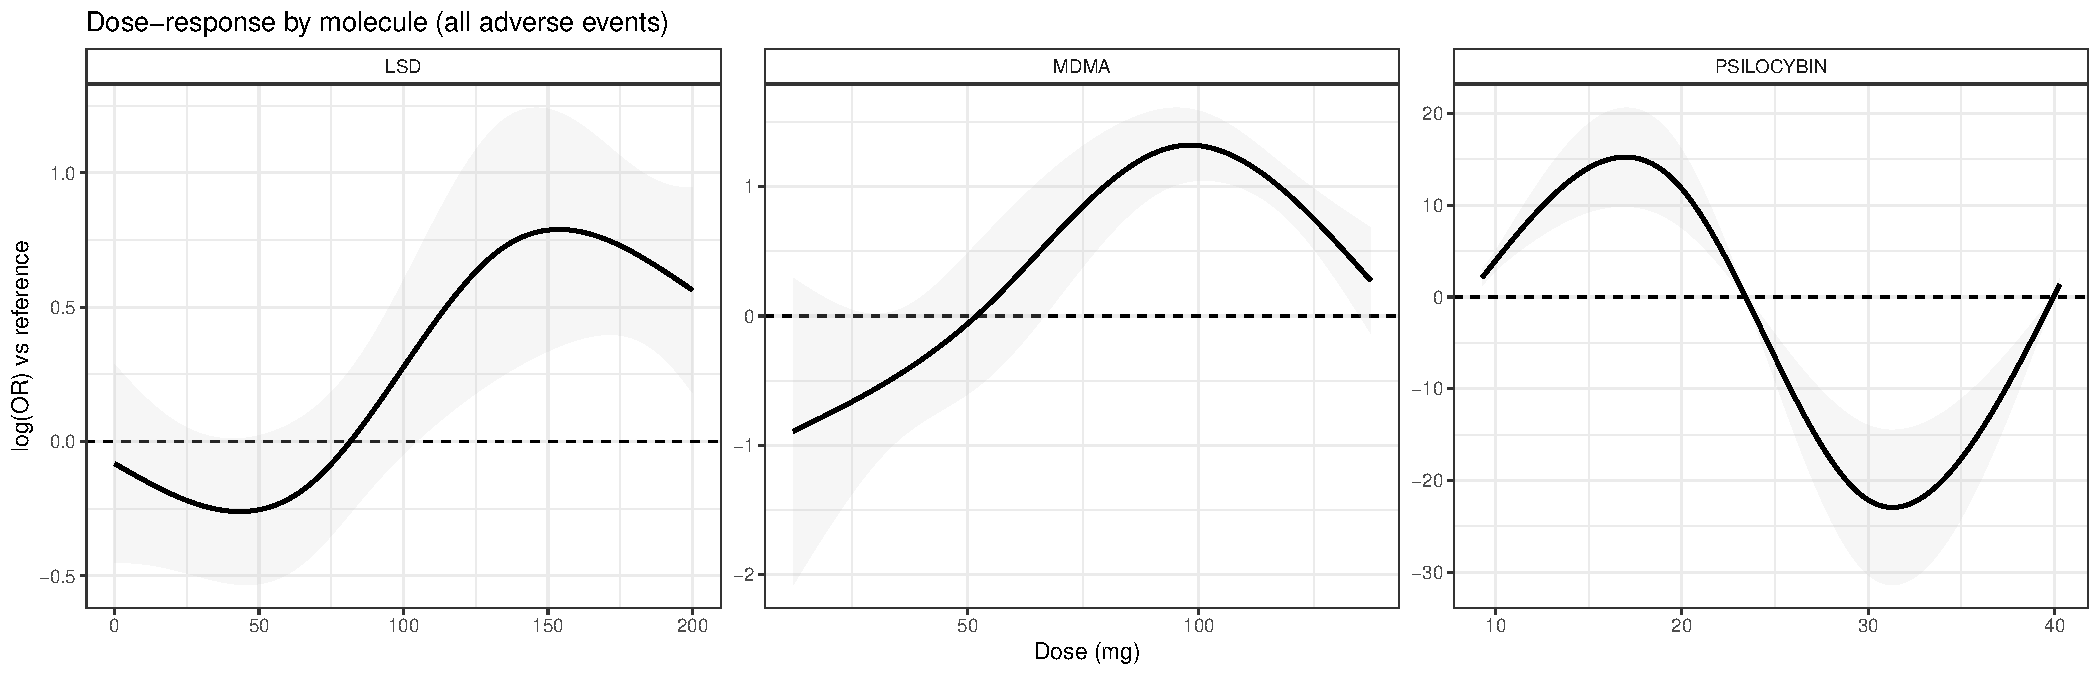
\includegraphics[width=\textwidth]{figures/master_dr_by_molecule-session.pdf}
  \caption{Global dose--response during session by molecule.}
  \label{fig:dr-global-session}
\end{figure}

\begin{figure}[htb]
  \centering
  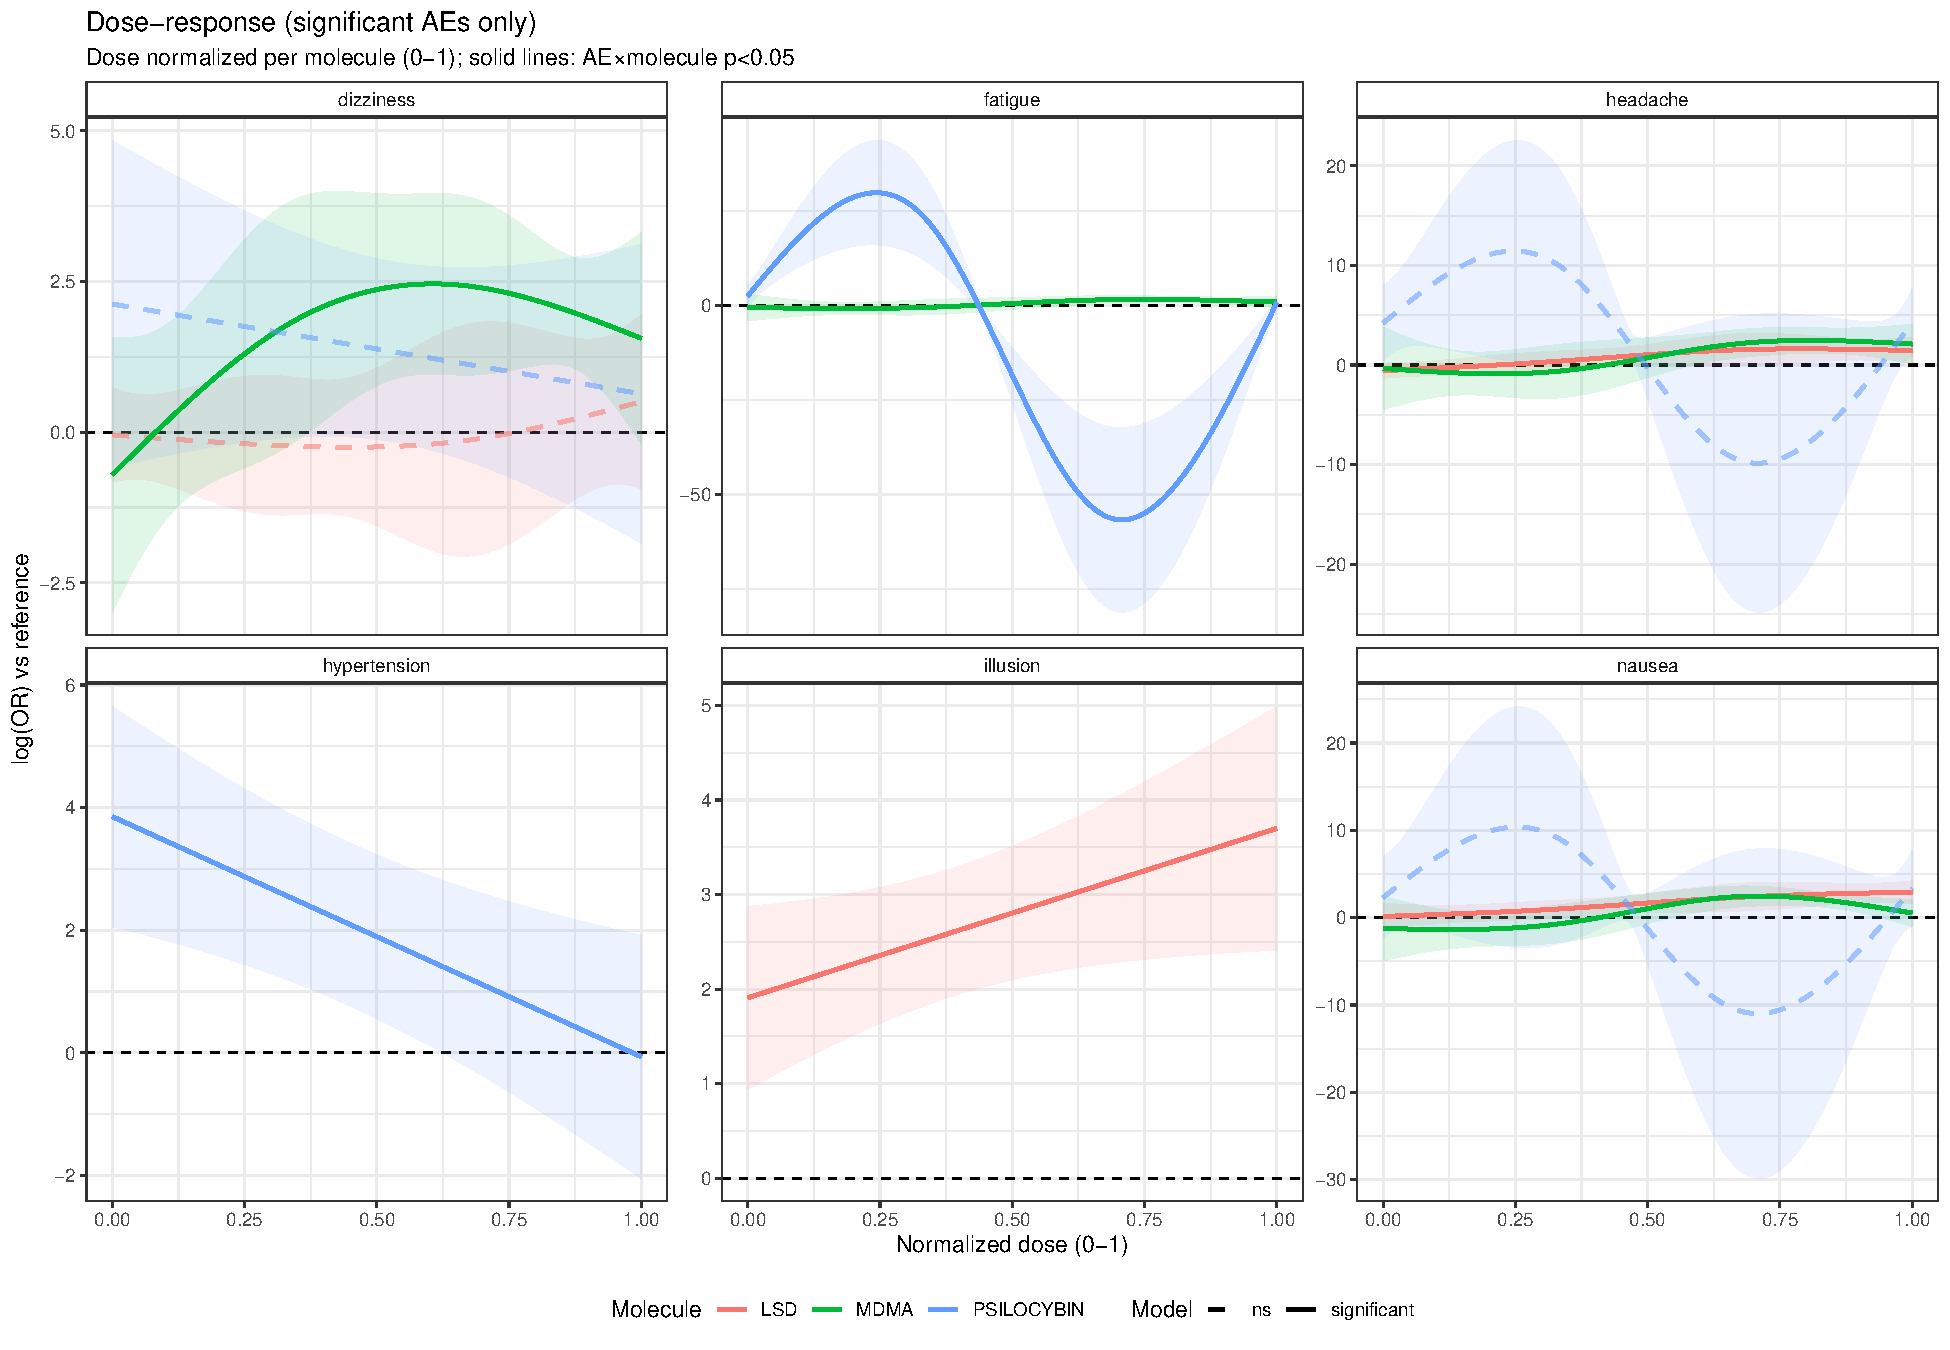
\includegraphics[width=\textwidth]{figures/master_dr_by_ae-session.pdf}
  \caption{Dose--response by adverse event (AE) during session (facets by molecule and AE).}
  \label{fig:dr-by-ae-session}
\end{figure}

\begin{figure}[htb]
  \centering
  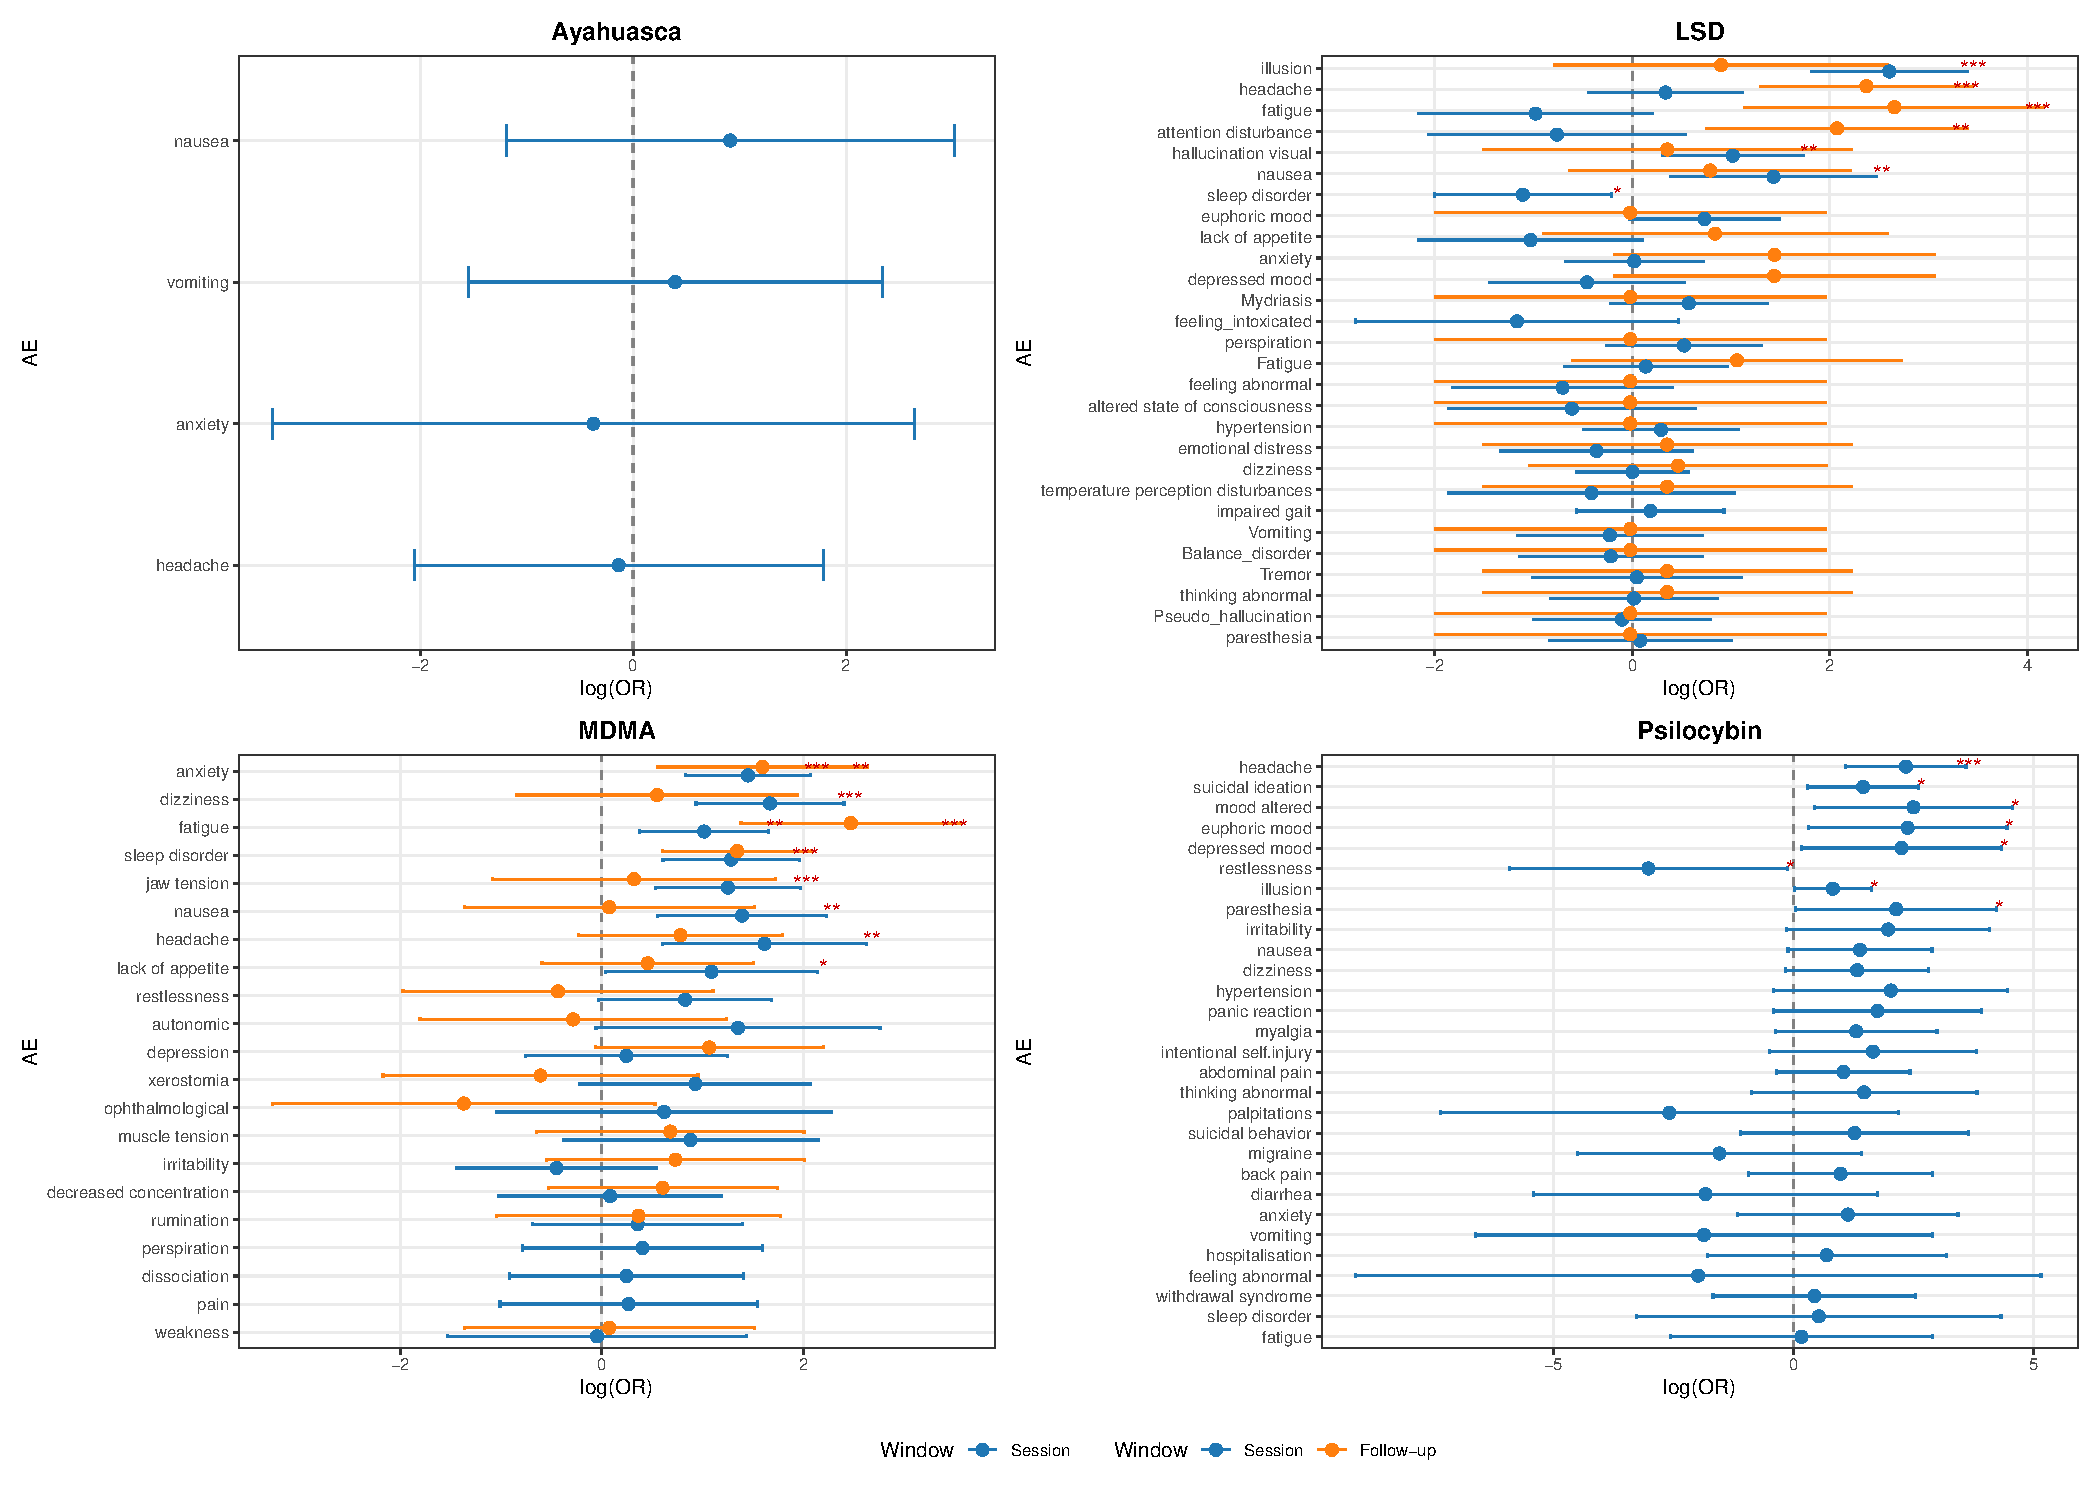
\includegraphics[width=\textwidth]{figures/forest_combined_all_molecules.pdf}
  \caption{Forest plots of AE odds ratios (OR) by molecule and time window (session vs follow-up).}
  \label{fig:forest-combined}
\end{figure}

\begin{table}[htbp]
  \centering
  \caption{Global session dose--response tests by molecule.}
  \label{tab:dr-global-by-molecule}
  \begin{tabular}{lcccc}
    \toprule
    Molecule & $k_{\text{session}}$ & $Q_M$ & $p$ & Sig. \\
    \midrule
    LSD & 149 & 11.36 & 7.49e-04 & *** \\
    MDMA & 197 & 5.16 & 2.31e-02 & * \\
    PSILOCYBIN & 162 & 19.13 & 1.22e-05 & *** \\
    \bottomrule
  \end{tabular}
\end{table}

\begin{table}[htbp]
  \centering
  \caption{Significant session dose--response effects by adverse event (AE) and molecule.}
  \label{tab:dr-ae-by-molecule-session}
  \begin{tabular}{llcc}
    \toprule
    Molecule & AE & $p$ & Sig. \\
    \midrule
    LSD & Nausea & 3.17e-03 & ** \\
    LSD & Headache & 1.04e-02 & * \\
    LSD & Illusion & 4.94e-02 & * \\
    MDMA & Headache & 4.95e-05 & *** \\
    MDMA & Dizziness & 4.87e-02 & * \\
    PSILOCYBIN & Fatigue & 2.54e-06 & *** \\
    PSILOCYBIN & Hypertension & 4.07e-03 & ** \\
    \bottomrule
  \end{tabular}
\end{table}

\begin{table}[htbp]
  \centering
  \caption{Significant pooled adverse event (AE) signals by molecule and assessment window.}
  \label{tab:ae-transition}
  \begin{tabular}{lllcl}
    \toprule
    Molecule & AE & Session $p$ & Follow-up $p$ & Temporal profile \\
    \midrule
    LSD & Nausea & 2.50e-02 & 8.85e-01 & Transient (session-only) \\
    LSD & Headache & 1.04e-02 & 6.29e-01 & Transient (session-only) \\
    MDMA & Depression & 4.56e-02 & -- & Session-only (no follow-up data) \\
    MDMA & Headache & 6.54e-03 & -- & Session-only (no follow-up data) \\
    Psilocybin & Fatigue & 2.54e-06 & -- & Session-only (no follow-up data) \\
    \bottomrule
  \end{tabular}}
\end{table}

\begin{table}[htbp]
  \centering
  \caption{Counts of significant adverse events (AEs) by temporal profile (p\,$<0.05$ in forest models).}
  \label{tab:forest-ae-sig-counts}
  \begin{tabular}{lccccc}
    \toprule
    Molecule & AE sig. (Session) & AE sig. (Follow-up) & Transient & Emergent & Persistent \\
    \midrule
    LSD & 4 & 3 & 4 & 3 & 0 \\
    MDMA & 8 & 3 & 5 & 0 & 3 \\
    PSILOCYBIN & 8 & 0 & 8 & 0 & 0 \\
    \midrule
    Total & 20 & 6 & 17 & 3 & 3 \\
    \bottomrule
  \end{tabular}
\end{table}

